\chapter{Fremgangsmåde i projektet}
Til støtte for gennemførelse af dette projekt udarbejdes først en handlingsplan bestående af følgende elementer:
\begin{enumerate}
 \item Målsætning for projektet. Målsætningen neddeles i:
  \begin{enumerate}
   \item en formåls-beskrivelse,
   \item en liste over leverancer i projektet og
   \item projektets succeskriterier
  \end{enumerate}
 \item Projektafgrænsning
 \item Interessentanalyse
 \item Milestone-plan
 \item Projektorganisation
 \item Arbejdsrum
\end{enumerate}

\section{Projektets målsætning}
For at lave afgangsprojektet har vi behov for en klar målsætning.\\

Telekommunikationen netværket i Grønland (især i nordgrønland og østgrønland) er nu ved at være forældet. Derfor har Tele Greenland planer om at udskifte den nuværende kommunikationsnetværk med nyere teknologi, som opfylder kundernes behov. Tele Greenland har allerede i dag nyere kommunikationssystem i nogle steder i Grønland, især i større befolkede byer. Det teknologi skal udvides og fornyes i nogle steder. I mindre befolkede byer som i nordgrønland, skal hele kommunikationssystemet skiftes. Planen er at det nye kommunikationsnetværk kun skal være “mobile only", dvs. den fastnette kommunikationssystem bliver udfaset.

\subsection{Formålsbeskrivelsen}
\emph{Vi ønsker at afklare, hvorledes Tele Greenland's forbindelser mellem kunden og centralen i bygder og mindre byer kan udskiftes fra kabelforbindelser til trådløse forbindelser.}\\

Følgende emner bliver analyseret:
\begin{itemize}
	\item Størrelsen af Grønland
	\item Befolkningstal
	\item Hvilke produkter/services kunderne bruger i hver by og hver bygd
\end{itemize}

For at projektet leveres og afsluttes tilfredsstillende er der lavet succeskriterier, som kan læses i afsnit \ref{succes} 

%Ud fra analysen undersøges følgende for at opfylde den nuværende og fremtidige behov af:
%\begin{itemize}
%	\item Udbredelsen af signalet
%	\item Datarater
%	\item Produkter og services 
%\end{itemize}
%
%Ud fra analysen, sættes der krav til det nye kommende kommunikationssystem. Der skal stilles krav til hvor antennerne skal placeres, hvor stor udbredelsen skal være, datarater og hvilke produkter/services der skal udbydes til kunderne.\\\\
%
%Inden der begyndes at regne på forskellige ting, afgrænses der fra følgende:
%\begin{itemize}
%	\item Kun en bygd eller en region med flere bygder bliver kigget på
%	\item Der vil kigges på udbredelsen og opnåelige datarater og ikke kommunikationstyper
%	\item Udvandring fra bygderne og mindre byer tages ikke højde for
%\end{itemize}



\subsection{Projektets leverancer}
Projektets leverancer er en Rapport - færdiggjort og afleveret inden den 5. januar kl. 12.00 (dansk tid) 2017 indeholdende:
\begin{itemize}
	\item Case-study af én eller to udvalgte bygder
	\item 
\end{itemize}                                                                                                         

\subsection{Projektets succeskriterier}\label{succes}
Projektet har to sæt succeskriterier. Det ene sæt er kriterierne for en god projektrapport, der bliver evalueret ved afgangseksamen. Her skal rapporten demonstrere, at den studerende:
\begin{itemize}
 \item "Skal kunne vurdere praksisnære og teoretiske problemstillinger samt begrunde og vælge relevante løsningsmodeller.”
 \item ”Skal evne at omsætte akademiske kundskaber og færdigheder til relevant, praktisk problembearbejdning og løsning på diplomingeniørniveau”
 \item "Skal evne at opstille robuste tids- og arbejdsplaner for eget projekt”
 \item ”Skal selvstændigt og med professionel tilgang kunne indgå i en dialog med professionelle interessenter”
\end{itemize}
\par

Det andet sæt succeskriterier er kriterierne for en anvendelig løsning, der opfylder formålsbeskrivelsen. Følgende succeskriterrier sættes op:
\begin{itemize}
%	\item Anlæg og drift af det valgte "wireles-last-mile"-koncept skal være billigere end renovering af det udslidte kabel-net i bygderne og de mindre byer - set over 5 år.
	\item Udarbejdelse af prognose for kapacitetskrav
	\item Udarbejdelse af specifikationer for, hvilke interfaces/tjenester, det trådløse Last-Mile koncept skal levere
	\item Ud fra kapacitetskrav udarbejde krav til dimensionering af det lokale mobilnet ()
	\item Identifikation af, hvilke informationer, der er nødvendige for at kunne beregne eller analysere kapacitet og dækningsbehov på en given lokation
	\item Udarbejde en model og en metode, som kan bruges til at beregne placering, antal og typer af antenner - En beregningsmodel som efterfølgende kan genbruges generelt på en given lokation.
	\item beskrivelse af de værktøjer, der anvendes for - ud fra modellen - at 
	\item Udarbejdelse af specifikationer til valg af bygd, der er velegnet for en case-study (forslag: En bygd, hvor alle tjenester er repræsenteret, og hvor de topografiske forhold er en udfordring)
	\item Valg af bygd
\end{itemize}
\section{Interessentanalyse for projektet}
\emph{''Hvem skal vi gøre glade''}
I interessentanalysen findes en liste over projektens interessenter, og en beskrivelse af hvordan interessenterne gøres tilfredse og hvordan de hvert enkel kommer til at bidrage til projektet.

\subsection{Liste over interessenter}

\begin{description}
 \item [A. Troels Bundgaard Sørensen] Associate Professor i Dep.8 (Department of Electronic Systems), Aalborg Universitet, +45 9940 8618\\
  \emph{Vejleder for Aqqalu Josefsen. Sidder i projektets styregruppe}.
 \item [B. John Siegstad (JFS)] Afdelingschef for afd.4400 Planning, Tele Greenland A/S, +299554853\\
 \emph{Sidder i projektets styregruppe.}
 \item [C. Haukur Thor Bragason (THOR)] Afdelingschef, Tele Greenland A/S, +299555224\\
  \emph{Teknisk ansvarlig for "Last Mile" i Grønland (dog ikke kabelnettet og krydsfelterne).}
 \item [D. Jukka Wagnholt (JUW)] Radioplanlægger, 386335, Tele Greenland A/S, +299585688\\
 \emph{Planlægger af Grønlands mobilnet. Anvender et Radio Planning og optimerings software udviklet af software-virksomheden "Forsk". Kan potentielt bidrage rigtig meget til projektet.}
 \item [E. ArKalo Andersen (ARAN)] Afdelingschef for afd.6020 TED LTS ("liniefolkene"), Tele Greenland A/S, +299562263\\
  Teknisk ansvarlig for land-kabelnettet og krydsfelterne.\\
  \emph{Det videre udfald , der efterfølger dette afleveringsprojekt, vil have indflydelse på hvordan og hvornår Wireless Last Mile erstatter kabelnettet i grønlandske bygder og mindre byer, hvilket igen vil have stor indflydelse på liniefolkenes arbejdsområde.}
  \item [F. Karin G. Nielsen (KGN)] Tegnestueleder, Tele Greenland A/S, +299550915.\\
   \emph{Forventes at kunne levere dokumentation som kort, tekniske tegninger og topografiske data til projektet.}
  \item[G. Mattias Törnquist (MATOR)] Planlægningsingeniør i afd.4120 4120 Server/ Database, Tele Greenland A/S +299386485\\
   \emph{Forventes at kunne levere statistiske data som antal abonnenter, kapacitetsforbrug, fremskrivninger o.lign.} 
\end{description}

\begin{figure}[!h]
	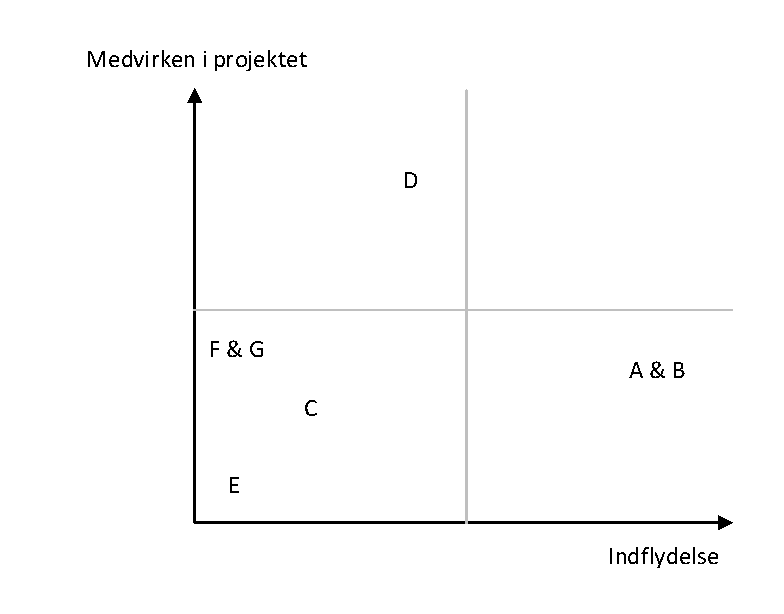
\includegraphics[width=1\textwidth]{interessentanalyse.pdf}
	\caption{Illustration af hvor interessenterne er placeret i forhold til medvirken og indflydelse for projektet}
\end{figure}



